\chapter{Technologie wykorzystane w implementacji}
  
  W poprzednim rozdziale opisano główne założenia proponowanego systemu i jego poszczególne funkcjonalności. W tym rozdziale zostaną opisane narzędzia, technologie i biblioteki, które zastosowano podczas budowy prototypu.

  \section{Zarys technologii}
    
    Implementację systemu oparto o technologie Java/Jee i pochodne. Jako podstawę szkieletu aplikacji wykorzystano framework Grails umożliwiający szybkie prototypowanie aplikacji internetowych. W warstwie bazy danych wykorzystano bazę postgresql oraz technologię mapowania obiektowo-relacyjnego Hibernate ORM, dostarczaną wraz z frameworkiem Grails. 
    
    Interfejs użytkownika oparto o Twitter Bootstrap - predefiniowany zestaw styli oraz komponentów do natychmiastowego wykorzystania w aplikacjach internetowych. 

    Moduł graficznej edycji diagramów UML został stworzony wykorzystując ,,jsUML2'' - bibliotekę przygotowaną przez zespół prof. José Raúl'a Romero, na uniwersytecie w Kordobie [!ref]. 

    Edytor tekstu oparty jest o bibliotekę javascript Ace Editor. Jest to wiodąca biblioteka, wykorzystywana m. in. w eksperymencie Cloud9 IDE [!ref] - webowym, zintegrowanym środowisku programistycznym zapoczątkowanym przez zespoł Mozilli, pod nazwą Mozilla Skywriter [!ref].
  
    Pierwotnie docelowym środowiskiem testowym dla proponowanego systemu był Google App Engine, jednak ze względu na ograniczenia tej usługi, prototyp umieszczono na darmowej infrastrukturze firmy Heroku (heroku.com) znacznie lepiej obsługującej nowoczesne aplikacje oparte o Javę.

  \section{Framework Grails}
    
    Framework Grails jest stosunkowo młodą technologią opartą na sprawdzonych rozwiązaniach. Firma która zajmuje się rozwojem tej technologii jest tą samą organizacją, odpowiedzialną za stworzenie Spring Framework - jednego z najpopularniejszych i jednocześnie najbardziej rozbudowanych platform programistycznych dla języka Java dostępnych na rynku. To właśnie Spring Framework leży u podstaw Grails i wraz z Hibernate ORM stanowi trzon technologiczny tego narzędzia.

   Grails integruje najlepsze praktyki i narzędzia zarówno ze Spring Framework jak i z Hibernate ORM. Jest poniekąd odpowiedzią środowiska Javy, na rosnącą konkurencyjność frameworków opartych o dynamicznie typowane, skryptowe języki programowania jak Django (język python) czy Ruby On Rails (Ruby). Jednocześnie, ze względu na fakt iż jest swoistą nakładką na technologie oparte na javie, dostarcza znacznie większych możliwości niż konkurenci, wynikających z rozbudowanego ekosystemu javy.


    \subsubsection{Język Groovy}

      Podstawowym językiem programowania w platformie Grails, jest język Groovy. Groovy jest dynamicznie kompilowanym językiem o składni i filozofii zbliżonej do takich języków jak Python lub Ruby. Kod bajtowy będący wynikiem kompilacji uruchamiany jest na wirtualnej maszynie Javy, przez co język integruje się niemal w sposób przeźroczysty z technologiami opartymi o JVM. Ponadto, kod programu napisanego w Javie jest poprawnym programem Groovy zarówno pod względem sytnaktycznym jak i semantycznym. Bardziej zwięzła i przyjazna składnia Groovy wraz z szerokimi możliwościami Javy sprawia, że ten język skryptowy jest solidnym rozwiązaniem o szerokim spektrum zastosowań.

      W celach porównawczych, poniżej zamieszczono znany, trywialny problem programistyczny ,,FizzBuzz'', zarówno w języku Groovy, jak i Java. Program ,,FizzBuzz'' otrzymując na wejściu ciąg liczb, wypisuje na konsolę słowo ,,Fizz'' jeśli dana liczba jest podzielna przez 3, słowo ,,Buzz'', jeśli dana liczba jest podzielna przez 5, natomiast słowo ,,FizzBuzz'' w przypadku podzielności przez 15.

    \begin{verbatim}

      // Groovy:
      for (i in 1..100) {
        println "${i%3?'':'Fizz'}${i%5?'':'Buzz'}" ?: i
      }    

      //Java:
      public class FizzBuzz{
        public static void main(String[] args){
          for(int i= 1; i <= 100; i++){
            if(i % 15 == 0){
              System.out.println("FizzBuzz");
            } else if(i % 3 == 0){
              System.out.println("Fizz");
            } else if(i % 5 == 0){
              System.out.println("Buzz");
            } else{
              System.out.println(i);
            }
          }
        }
      }

    \end{verbatim}

    \subsubsection{Grails}

    W szczególności filozofia Grails jest bardzo zbliżona do popularnego frameworka Ruby On Rails (RoR) umożliwiającego ekspresowe prototypowanie aplikacji obsługujących komunikację z bazą danych w zakresie (1) tworzenia, (2) odczytu, (3) aktualizacji i (4) usuwania danych za pomocą formularzy. Tego typu aplikacje popularnie nazywane są aplikacjami ,,CRUD'' - create, retrieve, update, delete). Wiele przyjętych rozwiązań w Grails zostało zaczerpniętych z RoR, jednak oba frameworki znacznie różnią się pod względem technologicznym. Szczegółowe porównanie tych technologii leży poza zakresem tej pracy, jednak osoby zainteresowane, powinny zapoznać się z doskonałym wątkiem w serwisie Stackoverflow, przytoczonym w bibliografii \cite{RailsGr}.


    Grails jest silnie oparte o paradygmat ,,convention over configuration'' - architekturze zakładającej minimalizację potrzeby konfiguracji aplikacji przez programistę na rzecz przyjętych konwencji, do których należy się stosować, aby wydaje dostarczać działające rozwiązania. Podejście to dotyczy wszelkich aspektów związanych z tworzeniem aplikacji w Grails - od struktury katalogów, przez umiejscowienie i zawartość plików konfiguracyjnych, po nazewnictwo klas, zmiennych i zastosowanie odpowiednich struktur danych. 

    \subsubsection{Model - View - Controller}

    Oparcie warstwy webowej w Grails na wzorcu Model-View-Controller (MVC) jest naturalnym podejściem w nowoczesnych frameworkach ułatwiających tworzenie aplikacji internetowych. Wzorzec MVC \cite{GoF} pierwotnie dotyczył tworzenia aplikacji okienkowych w Smalltalk'u-80 \cite{coad93}. Podstawowym założeniem MVC jest separacja danych i logiki od ich reprezentacji graficznej. MVC składa się z trzech rodzajów obiektów. 
  
    Model jest reprezentacją danych, wiedzy. Model może być odpowiednikiem jakiegoś obiektu lub strukturą wielu obiektów. 

    Widok jest wizualną reprezentacją modelu, ,,pobiera'' dane na temat obiektu i wyświetla je w odpowiedni sposób, często uwydatniając pewne elementy modelu, inne z kolei odpowiednio ukrywając. Funkcja ta czyni z widoku pewnego rodzaju filtr prezentacji danych. 

    Kontroler stanowi łącznik pomiędzy użytkownikiem a systemem, z którym użytkownik wchodzi w interakcję. Dostarcza użytkownikowi odpowiednich widoków, adekwatnych do stanu systemu \cite{Trygve79}.

    \begin{figure*}[t]
      \centering
      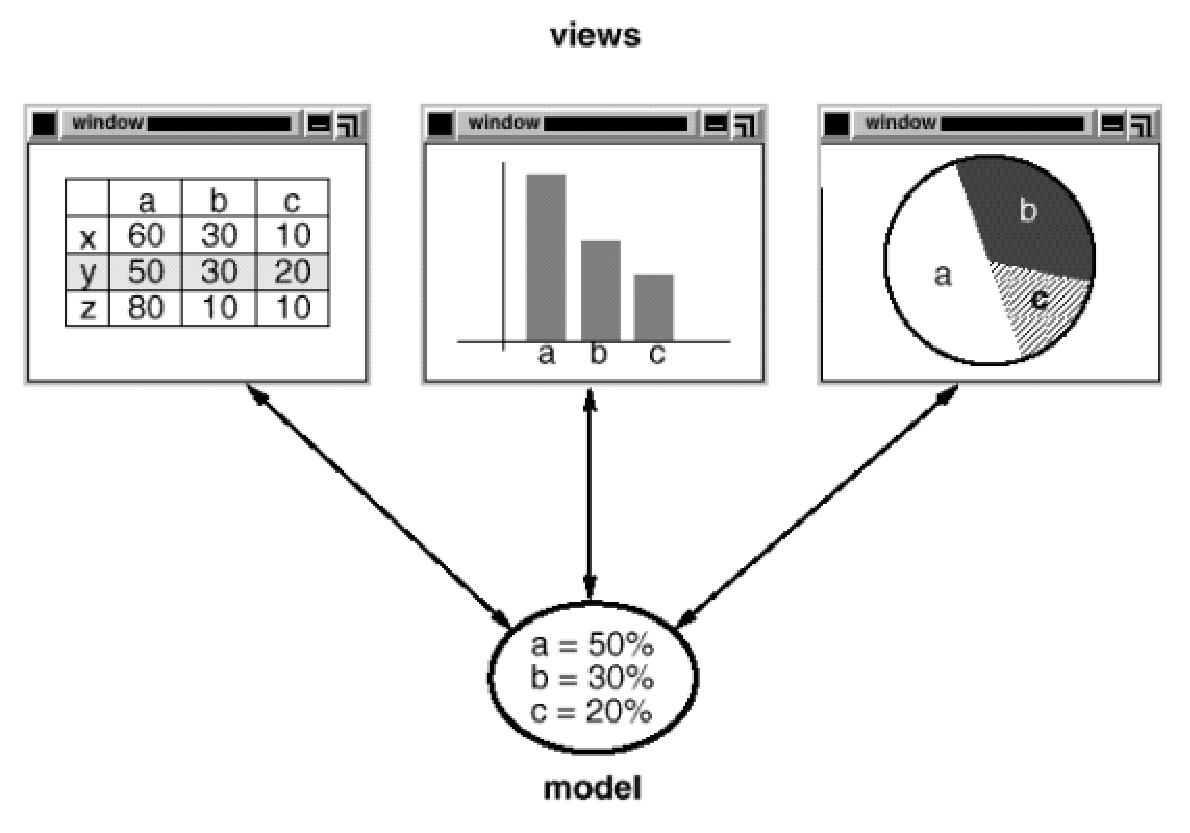
\includegraphics[width=1.0\textwidth]{img/mvc-1.pdf}
      \caption{Model-View-Controller - różna reprezentacja graficzna tych samych danych. Żródło: \cite{GoF}.}
      \label{fig:mvc-1}
    \end{figure*}

    \subsubsection{Praca z Grails}

    Struktura katalogów nowo utworzonej aplikacji Grails wygląda następująco:

    \begin{verbatim}

    + grails-app
      + conf           ---> lokalizacja artefaktów konfiguracji
        + hibernate    ---> opcjonalne pliki konfiguracyjne hibernate
        + spring       ---> opcjonalne pliki konfiguracyjne spring 
      + controllers    ---> kontrolery aplikacji
      + domain         ---> klasy reprezentujące modele
      + i18n           ---> zlokalizowane komunikaty il8n
      + services       ---> warstwa serwisowa
      + taglib         ---> biblioteki znaczników
      + util           ---> klasy pomocnicze special utility classes 
      + views          ---> lokalizacja widoków
        + layouts      ---> lokalizacja 
      + lib
      + scripts       ---> scripts
      + src
      + groovy       ---> optional; location for Groovy source files
                            (of types other than those in grails-app/*)
      + java      ---> optional; location for Java source files
      + test          ---> generated test classes
      + web-app
        + WEB-INF

    \end{verbatim}

    \subsubsection{GORM - Grails Object Relational Mapping}
  
    Po wstępnej analizie, mając wiedzę na temat dziedziny problemu, w prosty sposób można utworzyć podstawową funkcjonalność przykładowej aplikacji. Proces tworzenia elementów budowanego systemu rozpoczyna się od stworzenia klasy Groovy reprezentującej model (na przykładzie implementacji z systemu Reqmanager):

    \begin{verbatim}
    package pl.edu.pjwstk.reqmanager.examples
    class Project {
        String name
        String description
        String mainNote
        java.sql.Timestamp timestamp
        java.util.Date deadline

        static hasMany = [requirements:Requirement]
    }
    \end{verbatim}

    Jeśli nie skonfigurujemy aplikacji w niestandardowy sposób, po stworzeniu powyższej klasy Groovy w katalogu grails-app/domain, Framework Grails przy pomocy Hibernate utworzy następującą strukturę w bazie danych:

    \begin{verbatim}
                      Table "public.project"
       Column    |            Type             | Modifiers 
    -------------+-----------------------------+-----------
     id          | bigint                      | not null
     version     | bigint                      | not null
     deadline    | timestamp without time zone | 
     description | character varying(255)      | not null
     name        | character varying(255)      | not null
     timestamp   | timestamp without time zone | not null
     main_note   | character varying(255)      | 
    Indexes:
        "project_pkey" PRIMARY KEY, btree (id)
    Referenced by:
        TABLE "requirement" CONSTRAINT "fk15a8dc43ffd118f2" 
        FOREIGN KEY (project_id) REFERENCES project(id)
    \end{verbatim}

    Powyższy przykład przedstawia, jak w prosty sposób, przy niskich nakładach pracy, programista jest w stanie zbudować szkielet aplikacji zasilanej bazą danych. Jak widać, pola klasy Groovy, zostały odpowiednio odwzorowane w strukturze danych wraz z odpowiednimi typami danych po stronie bazy.

    Na szczególną uwagę zasługuje konstrukcja w klasie Project: 

    \begin{verbatim}
      static hasmany = [requirements:requirement]
    \end{verbatim}

    W języku Groovy konstrukcja ,,[:]'' jest reprezentacją pustej tablicy asocjacyjnej - struktury danych umożliwiającej przechowywanie kolekcji par ,,klucz - wartość''. W Groovy, domyślną kolekcją inicjalizowaną przy pomocy literału ,,[:]'' jest obiekt klasy java.util.LinkedHashMap. Zatem powyższa zmienna statyczna jest referencją do obietku klasy LinkedHashMap, zawierającego jedną parę, gdzie kluczem jest ciąg znaków ,,requirements'' a wartością, jest klasa Requirement. W ten sposób Grails obsługuje relacje jeden-do-wielu. W analogiczny sposób, istnieje możliwość definiowania pozostałych rodzajów relacji, tj. jeden-do-jeden, wiele-do-wielu, etc). Konstrukcja taka, umożliwia uzyskanie listy wymagań w projekcie: 

    \begin{verbatim}
      //pobiera z bazy projekt o id = 1
      def project = Project.get(1)

      //zwraca listę wymagań podłączonych do projektu
      def reqs = project.requirements 
    \end{verbatim}
    
      
    \subsubsection{Kontrolery i widoki}

    W celu połączenia konkretnych widoków z akcjami kontrolerów, konwencja Grails wymaga odpowiedniego nazewnictwa metod w klasach kontrolerów. Generalizując, należy stosować się do zasady, aby nazwa metody odpowiedzialnej za realizację wybranej akcji kontrolera, posiadała plik o tej samej nazwie, z rozszerzeniem .gsp, w odpowiednim katalogu w ścieżce grails-app/views. Poniżej zamieszczono przykład realizacji akcji ,,index'' w kontrolerze ,,ProjectController''. Wbudowany w Grails mechanizm odwzorowywania adresów URL i przekierowywania do odpowiednich akcji kontrolerów automatycznie wykrywa którą metodę należy wykonać. Zatem, po wskazaniu przeglądarce internetowej adresu http://reqmanager.heroku.com/project/index system, przez konwencję, wykryje konieczność wywołania metody ,,index'' w kontrolerze ,,ProjectController''. Z kolei po wykonaniu tej metody, (o ile programista nie zdecyduje inaczej) automatycznie wyświetlany jest widok index.gsp umieszczony w katalogu grails-app/views/project. W widoku, do wykorzystania dostępne są zmienne usatwione w tabeli asocjacyjnej, zwracanej przez kontroler (w tym przypadku, zmienna ,,project'' zawierająca referencję do listy wszystkich projektów w systemie). 


    \begin{verbatim} 
      // klasa kontrolera:
      package pl.edu.pjwstk.reqmanager

      class ProjectController {
        def index = { 
          return [projects : Project.list()]
        }   
      }

      //widok w pliku o nazwie index.gsp 
      //umieszczony w katalogu grails-app/views/project/
      <!DOCTYPE html>
      <html>
        <div>
        <h1>Project list</h1>
        <g:each in='${projects}' var='project'>
          Nazwa: ${project.name}<br />
          Deadline: ${project.deadline.format("dd-MM yy")}<br />
          Opis: ${project.description} 
        </g:each>
        </div>
      </html>

    \end{verbatim}

    Należy jeszcze zwrócić uwagę na pewien detal w strukturze kodu źródłowego kontrolera. Grails dopuszcza dwa podejścia do deklarowania akcji - (1) za pomocą klasycznych metod oraz (2) przy użyciu dokmnięć (closures). Formalnie domknięcia są obiektami wiążącymi funkcję oraz środowisko w jakim ta funkcja ma działać. Jest to specyficzna kontrukcja, będącą zdefiniowanym blokiem kodu, który można przekazać jako parametr innej metodzie lub funkcji. Poniższy przykład wyjaśnia zasadę na jakiej działają domknięcia w Groovy: 
    
    \begin{verbatim}
      def closeAllProjects() {
        def projects = Project.list()
        projects.collect { it.open = false }
      }
    \end{verbatim} 
    
    Powyższy kod pobiera do zmiennej ,,projects'' listę wszystkich projektów w systemie. Następnie, na liście projektów wywoływana jest metoda ,,collect''. Metoda collect (zdefiniowana w interfejsie Collection) przyjmuje jako parametr blok kodu, domknięcie. Metoda collect iteruje po wszystkich elementach zbioru na rzecz którego jest wykonana i wykonuje blok kodu na kolejnych elementach kolekcji przekazany jej jako parametr, następnie zwracając listę zmodyfikowanych przez domknięcie elementów.

    \subsection{Spring Framework i Hibernate ORM}

      Sercem Grails jest Spring Framework oraz Hibernate ORM. Obie technologie są wiodące na rynku i szeroko stosowane w komercyjnych projektach dowolnych rozmiarów. Spring jest de facto zestawem narzędzi, wzorców projektowych i bibliotek realizujących ogromną ilość funkcjonalności, mających za zadanie przyśpieszyć proces wytwarzania oprogramowania oraz w pewnym zakresie zapewnić wysoką jakość tworzonych rozwiązań. Przede wszystkim jednak, jest tzw. kontenerem Inversion Of Control (odwrócenie sterowania) \cite{MFow01}. ********** tu trochę o IoC ***********. Prócz IoC Spring Framework to potężna platforma integrująca wiele rozwiązań, takich jak webowy framework Spring MVC, biblioteki i wzorce dotyczące bezpieczeństwa (Spring Security), wrapper jdbc, transakcje (Spring JDBC Templates), etc.

      Hibernate ORM jest technologią pozwalającą na mapowanie rekordów z relacyjnych baz danych, na obiekty w systemie. Jest to metoda w pewnym stopniu rozwiązująca problem niezgodności impedancji \cite{KSub01}

  \section{Pozostałe technologie}
    \subsection{Postgresql}
      Trwałość danych w aplikacjach internetowych standardowo realizowana jest przez bazę danych. Na potrzeby prezentowanego prototypu, wykorzystano bazę danych Postgresql. Jest to obiektowo-relacyjna baza danych udostępniona na licencji Wolnego i Otwartego Oprogramowania. 

      Baza danych PostgreSQL implementuje znaczną część standardu SQL:2008 [!ref - http://www.postgresql.org/docs/9.1/static/features.html]

    \subsection{Javascript, jQuery i biblioteka jsUML2}

      Wiele funkcjonlaności zrealizowano po stronie klienta, wykorzystując język javascript. W niewielkim zakresie wykorzystano popularną bibliotekę jQuery, wspierającą realizację najczęściej pojawiających się problemów w trakcie prac nad aplikacjami intenretowymi. Jednak wykorzystanie jQuery w prototypie systemu jest marginalne i ogranicza się jedynie do zastosowania metody \emph{ajax()} ułatwiającej wykonywanie asynchronicznych wywołań serwera.

      \subsubsection{jsUML2}
        jsUML2 jest biblioteką stworzoną na uniwerystecie w Kordobie. Jest to zaimplementowany w całości w języku javascript, rozbudowany zestaw klas umożliwiający tworzenie wielu rodzajów diagramów UML w przeglądarce internetowej. jsUML wykorzystuje najnowszą specyfikację języka znaczników HTML5. Obiekt \emph{canvas} oferuje szerokie spektrum możliwości programistom aplikacji internetowych. Element \emph{canvas} umożliwia programistyczne tworzenie kształtów i obrazów bitmapowych w przeglądarce internetowej. Canvas udostępnia programistom interfejs HTMLCanvasElement umożliwiający modyfikację zawartości elementów canvas w htmlu. Metoda interfejsu \emph{getContext()} zwraca tzw. ,,drawing context''.... 
        
      
       
    \subsection{System kontroli wersji git i serwer heroku}
    \subsection{Srodowisko programistyczne (linux, vim, tmux)}
